


\section{Simulating Shapes}


A very important issue in computational physics is dealing with particles and objects of arbitrary shapes interacting with each other. There are many possible solutions for this problem, depending on the shapes that one wants to simulate. In some very special cases, like ellipsoidal particles, it is possible to find analytic solutions for the equations of motion.



\subsection{Ellipsoidal particles}

The general parametrisation of two ellipses (see Fig. \ref{fig:ellipses}) in 2D is given by the equations

\begin{align*}
\kl{\frac{x-x_a}{a_1}}^2 + \kl{\frac{y-y_a}{a_2}}^2 &= 1\\
\kl{\frac{x-x_b}{b_1}}^2 + \kl{\frac{y-y_b}{b_2}}^2 &= 1
\end{align*}


Perram and Wertheim \citep{perram} proposed to take the overlap of the shapes as a measure for the interaction. To calculate the overlap one can transform the ellipses into circles using an appropriate metric \citep{comp_phys}. We can generalize an ellipse with the functional 
\begin{equation}
G_A\kl{\vec{r}} = \kl{\vec{r}-\vec{r}_a}^{\,T} \mat{A} \kl{\vec{r}-\vec{r}_a}
\label{eq:ellipse_func}
\end{equation}

which is smaller than one inside the ellipse, larger then one outside and exactly one on the ellipse:

\begin{equation}
G_A\kl{\vec{r}} =\begin{cases}
  <1,  & \text{if } \vec{r} \text{ is inside the ellipse}\\
  \,\,\,\,\,\,1,  & \text{if } \vec{r} \text{ is on the ellipse}\\
  >1,  & \text{if } \vec{r} \text{ is outside the ellipse}
\end{cases}
\end{equation}



\vspace{0.1cm}
\noindent
\begin{minipage}{\textwidth}
\begin{minipage}{.85\textwidth}
  \centering
  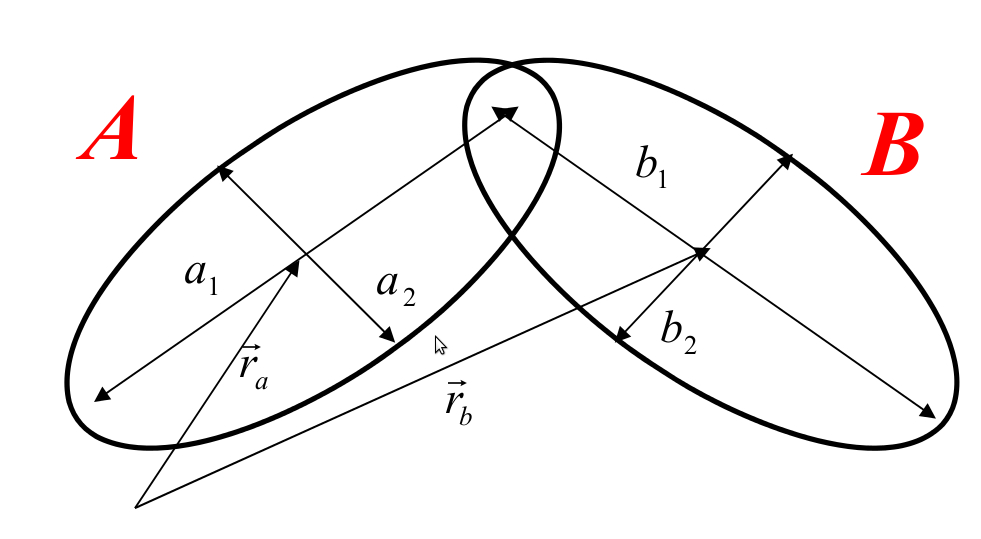
\includegraphics[width=.85\textwidth]{pics/ellipses.jpg}
  \captionof{figure}{Parameters for the characterization of two ellipses.}
  \label{fig:ellipses}
\end{minipage}
\hfill
\begin{minipage}{.001\textwidth}
 \end{minipage}
\end{minipage}
\vspace{0.1cm}

We can now define a new joint functional for the two ellipses that is weighted with a parameter $\lambda$ that interpolates between the two centers of the ellipses defined with \eqref{eq:ellipse_func}. $\lambda$ goes from 0 to 1, and in the extrema the functional signs the centre of the first or the second ellipse respectively.

\begin{equation}
G\kl{\vec{r},\lambda} = \lambda G_A\kl{\vec{r}}  + \kl{1-\lambda} G_B\kl{\vec{r}} 
\end{equation}

For every $\lambda$ we have a surface, and for every $\lambda$ we are interested in the minimum of the surface. To find the minimum we have to minimize the functional:
\begin{equation*}
\nabla_{\vec{r}}\,G\kl{\vec{r},\lambda} = 0.
\end{equation*}
which yields
\begin{equation}
\vec{r}_m \kl{\lambda} = \kl{\lambda \mat{A} + \kl{1-\lambda} \mat{B}}^{-1} \kl{\lambda\mat{A}\vec{r}_a + \kl{1-\lambda}\mat{B}\vec{r}_b}.
\end{equation}
If we start from $\lambda=0$ and arrive to $\lambda=1$ we will get a path from the center of the first ellipse to the other. We can rewrite the path defining $\vec{r}_{ab}\equiv \vec{r}_b-\vec{r}_a$ and obtain

$$
\vec{r}_m \kl{\lambda} = \vec{r}_a +\kl{1-\lambda} \mat{A}^{-1} \ekl{  \kl{1-\lambda} \mat{A}^{-1} + \lambda \mat{B}^{-1}  }^{-1} \vec{r}_{ab}
$$
\begin{equation}
\vec{r}_m \kl{\lambda} = \vec{r}_b -\kl{1-\lambda} \mat{B}^{-1} \ekl{  \kl{1-\lambda} \mat{A}^{-1} + \lambda \mat{B}^{-1}  }^{-1} \vec{r}_{ab}
\label{eq:min_path}
\end{equation}

These paths are very handy: if the value of the functional along the path between the centers always smaller than 1, we know that we did not have to leave the ellipses, hence they overlap. We can define an \emph{overlap function} 
\begin{equation}
S\kl{\lambda} \equiv G\kl{\vec{r\kl{\lambda}},\lambda} 
\end{equation}
and if we insert \eqref{eq:min_path} we get
\begin{equation}
S\kl{\lambda} = \lambda \kl{1-\lambda} \vec{r}_{ab}^{\,T}\ekl{  \kl{1-\lambda}\mat{A}^{-1}+ \lambda \mat{B}^{-1}   }^{-1}\vec{r}_{ab}
\end{equation}
This now is the height of the minimal path that connects the two centers. As already mentioned, we are interested if the path ever assumes values larger than 1. If we maximize $S$, we will be able to tell if the ellipses are overlapping or not:


\begin{equation}
S\kl{\lambda_{\text{max}}} =\begin{cases}
  <1,  & \text{if the ellipses overlap}\\
  \,\,\,\,\,\,1,  & \text{if the ellipses touch}\\
  <1,  & \text{if the ellipses are separated}
\end{cases}
\end{equation}

With this knowledge we can also calculate the contact point, if the ellipses are stiff and we have to avoid the overlap through an (in)elastic collision. We set $S\kl{\lambda_{\text{max}}}$ to unity and find the contact point using \eqref{eq:min_path}. 


Ellipses can be generalized to so-called \emph{superellipsoids} \citep{superellipsoids} and the macroscopic effects of these generalizations are all but trivial \citep{mms}. Industrial engineering, fluiddynamics in biology (e.g. blood cells) and many other fields often rely on simulations of macroscopic particles, often ellipsoidal, and this is why this techniques have such a big resonance today.


We saw that even for the simplest generalization of spheres, it was already necessary to develop complex analytical methods. This significantly increase the computational complexity and the time consumption of the programs. For this reason, it is necessary to develop new approaches to handle objects of arbitrary shapes.
%13b -21min



\subsection{Polygons}


A particular class of macroscopic particles are those that can be described by polygons (e.g. rocks, sand grains, etc.).  In this case, a better measure for the repulsive forces is the overlap area (\emph{Cauchy elasticity}). The advantage of simple polygons is that the overlap area can be computed using simple geometries (e.g. dividing the area into triangles). However, between polygons there can be many different types of contacts, and in 3D the classification and the identification of all the types of contacts can be very cumbersome (see Fig. \ref{fig:poly_contact}).



\vspace{0.1cm}
\noindent
\begin{minipage}{\textwidth}
\begin{minipage}{.85\textwidth}
  \centering
  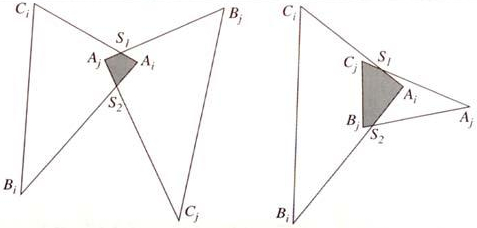
\includegraphics[width=.75\textwidth]{pics/poly_contact.jpeg}
 % \captionof{figure}{BLABLA.}
 % \label{fig:poly_contact}
\end{minipage}
\begin{minipage}{.85\textwidth}
  \centering
  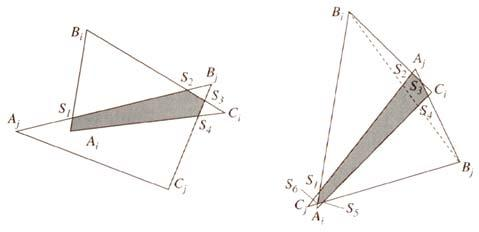
\includegraphics[width=.75\textwidth]{pics/poly_contact2.jpeg}
  \captionof{figure}{Possible overlaps of 2D Polygons.}
  \label{fig:poly_contact}
\end{minipage}
\end{minipage}
\vspace{0.1cm}







\vspace{0.1cm}
\noindent
\begin{minipage}{\textwidth}
\begin{minipage}{0.35\textwidth}
Additional complexities arise when the overlap area does not represent the actual overlap of the polygons (see Fig. \ref{fig:poly_contact4}, upper row) or discontinuities can appear while particles move into another (see Fig. \ref{fig:poly_contact4}, lower row). Furthermore, rotation of particles need additional treatment, as the torque strongly depends on the shape of the particles.
\end{minipage}
\begin{minipage}{0.65\textwidth}
\begin{minipage}{.85\textwidth}
  \centering
  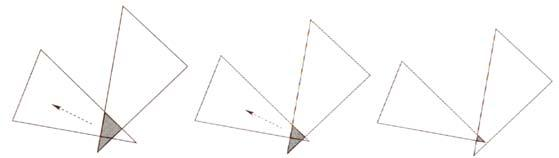
\includegraphics[width=.75\textwidth]{pics/poly_contact3.jpeg}
 % \captionof{figure}{BLABLA.}
 % \label{fig:poly_contact}
\end{minipage}
\begin{minipage}{.85\textwidth}
  \centering
  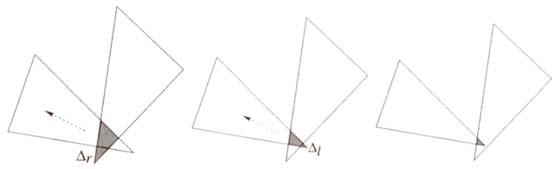
\includegraphics[width=.75\textwidth]{pics/poly_contact4.jpeg}
  \captionof{figure}{Possible issues with discontinuities.}
  \label{fig:poly_contact4}
\end{minipage}
\end{minipage}
\end{minipage}
\vspace{0.1cm}

Due to the mentioned reasons, the simulation of object composed of polygons can be tricky. In 3D, as always, things become horrible and the computation time for a large number of polyhedra increases enourmosly. 






\subsection{Spheropolygons}

% 13b -13


\vspace{0.2cm}
\noindent
\begin{minipage}{\textwidth}
\begin{minipage}{0.38\textwidth}
Another class of methods that are more efficient than the mere division into polygons  relies on \emph{spheropolygons} \citep{spheropolygons}. This technique was invented by Fernando Alonso-Marroquin, who uses the \emph{Minkowski cow} for demonstrative purpose. This particular shape is obtained by sweeping a disk around a polygon of multiple and arbitrary edges that resemble the shape of a cow (see Fig. \ref{fig:minkowski_cow}).
\end{minipage}
\hfill
\begin{minipage}{.58\textwidth}
  \centering
  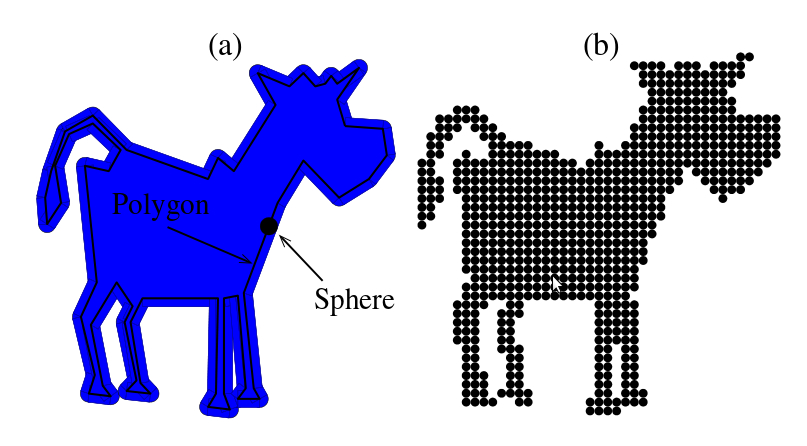
\includegraphics[width=.75\textwidth]{pics/minkowski_cow.jpeg}
  \captionof{figure}{Decomposition of a Minkowski cow into spheres}
  \label{fig:minkowski_cow}
\end{minipage}
\end{minipage}
\vspace{0.1cm}

The take-home message is that the shape can be arbitrary. Once the shape is decomposed into spheres one only has to compute the contact between all the pairs of spheres that compose the edges and vertices of the shape which is easier than considering arbitrary shaped polygons.  There are of course a number of constraints when approximating the shapes in such a way. For example, too large spheres would smear out the original shape excessively and would even yield wrong results. Imagine that the spheres at the edges were larger than the distance between the hooves or the distance between the tale and the rest of the cow. Substantial features of the shape would be lost. For further videos and information, see \cite{spheropolygons2}.


\vspace{1.5cm}
Nowadays, There are many other techniques to describe arbitrary shaped objects. Many attempts to create more effective implementations are developed by engineers, phycisists and mathematicians. An important example is the field of \emph{mathematical morphology} \citep{serra} developed by Jean Serra in the 1960s. The techniques of Marroquin are related to the so called \emph{dilation techniques} but there are also other methods like the \emph{erosion technique}. We will not go deeper into the variety of existing methods since their mathematical frameworks reach a point in which technicalities monopolizes entire lectures and even courses, such as \emph{Computational Science and Engineering}.












